\chapter{Results}
Several candidate satellites was studied before arriving at the one presented here. Spatiotemporal consistency and resolution was given high priority when choosing a dataset. Cloud mask are provided by all satellites, mostly because other retrievals are only possible under cloud free conditions. Humidity's is a good example of such a variable. 

The satellite product chosen for this thesis is the \acrfull{msg}. This is geostationary, has a exceptional temporal resolution. Knowing that the average lifetime of a cloud is 60min or less, it seems like a reasonable choice. \textbf{kilde Lohmann s.19} The finished dataset is named \acrfull{ecc}.

\section{Dataset}
This section presents the developed algorithms necessary for the compilation of the dataset European Cloud Cover, ECC. It is pieces together from two sources, ERA5 reanalysis and METeosat second generation cloud mask. This requires the regridding of one of them.

\subsection{Domain}
For this project the geographical domain has been restricted latitude $\in[30,50]$ and longitude $\in [-15, 25]$. The resulting dimensions of the grid becomes $81\times161$ pixels. \textbf{Why not larger part of domain. 1) You have included parts with ...  2) } Seemed like a reasonable start, to prove a concept. Figure \ref{fig:map} shows the region of Europe included in this dataset. Covering the Mediterranean areas.

\begin{figure}[h]
    \centering
    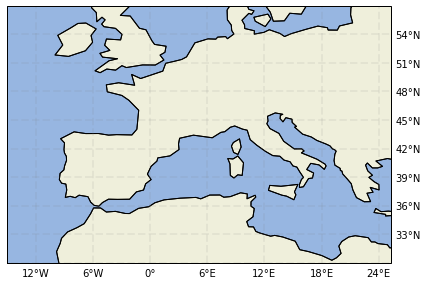
\includegraphics[scale = 0.7]{Chapter2_Theory/images/Domain.png}
    \caption{Map showing the domain. The region cover southern Europe and northern Africa. The coordinate system is Plate Caree, which is the same as ECC. The image have been generated using the python package cartopy ref? \textbf{new figure with correct range and some vegetation or topography on  } \textbf{generate new plot with the updated boundaries}}
    \label{fig:map}
\end{figure}

\subsection{European Cloud Cover} \label{sec:ecc}
\acrfull{ecc} comprises of five variables collected from two sources; ERA5 and EUMETSAT. Preserving the resolution available in ERA5, while remapping the cloud mask to cloud fractions. The final product consist of the variables temperature, pressure, cloud fraction, specific and relative humidity. Hourly data on a $0.25^o$ uniform grid resolution in the period \textbf{put in first date} to \textbf{last date}. Total cloud cover is produced from area weighting cloud masks. This computations are described in \ref{sec:remapping}. The others are on their original format as provided by \acrfull{ecmwf}. A summary of the original sources of the dataset is given in table \ref{tab:dataset_summary}. More details on ERA5 is available in Section \ref{sec:era5} and see section \ref{sec:EUMETSAT_cloud_mask} for more information about cloud mask. 
\begin{table}[]
    \centering
    \resizebox{\textwidth}{!}{%
\begin{tabular}{c|c|c|c|c|}
\cline{2-5}
\multirow{4}{*}{}                                 & \multicolumn{2}{c|}{\textbf{ERA5}}                                                                                                   & \multicolumn{2}{c|}{\textbf{MSG2}}                                                                                                                \\ \cline{2-5} 
                                                  & \textbf{Type}                     & \textbf{Variables}                                                                               & \textbf{Type}                                                               & \textbf{Variables}                                                  \\ \cline{2-5} 
                                                  & Surface                           & \begin{tabular}[c]{@{}c@{}}2m Temperature\\ Surface pressure\end{tabular}                        & \multirow{2}{*}{Satelite retrival}                                          & \multirow{2}{*}{Cloud Mask}                                         \\ \cline{2-3}
                                                  & 1000 hPa                          & \begin{tabular}[c]{@{}c@{}}Relative Humidity\\ Specific Humidity\end{tabular}                    &                                                                             &                                                                     \\ \hline
\multicolumn{1}{|c|}{\textbf{Projection}}         & \multicolumn{2}{c|}{Uniform grid}                                                                                                    & \multicolumn{2}{c|}{Curve linear grid}                                                                                                            \\ \hline
\multicolumn{1}{|l|}{\textbf{Spatial resolution}} & \multicolumn{2}{c|}{$0.25^o$}                                                                                                        & \multicolumn{2}{c|}{-}                                                                                                                            \\ \hline
\multicolumn{1}{|c|}{\textbf{Output Frequencey}}  & \multicolumn{2}{c|}{Hourly}                                                                                                          & \multicolumn{2}{c|}{15 min}                                                                                                                       \\ \hline
\multicolumn{1}{|c|}{\textbf{Availability}}       & \multicolumn{2}{c|}{\begin{tabular}[c]{@{}c@{}}1979-onwards\\ Expected to be available from \\ 1950 some time in 2020.\end{tabular}} & \multicolumn{2}{c|}{2004-onward}                                                                                                                 \\ \hline
\multicolumn{1}{|c|}{\textbf{License}}           & \multicolumn{2}{c|}{\begin{tabular}[c]{@{}c@{}}Open Access. Need user \\ from Copernicus Data Storage.\end{tabular}}                  & \multicolumn{2}{c|}{\begin{tabular}[c]{@{}c@{}}Researcher Licences\\ to get 15min resolution.\\ Open access at \\ hourly resolution\end{tabular}} \\ \hline
\end{tabular}
}
\caption{Data description on the data present in the dataset ECC (European Cloud Cover). \textbf{Add projection as a column, Availability for download and the period of data.} There is a lot of work in combining the two datasets and processing it.}
\label{tab:dataset_summary}

\end{table}

%%%%%%%%%%%%%%%%%%%%%%%%%%%%%%%%%%%%%%%%%%%%%%%%%%%%
\subsubsection{Physical basis of variable decision} \label{sec:physical_basis}
The overall goal is to investigate if its enough information to predict clouds in the meteorological variables such as temperature, pressure and humidity. On the one hand, like discussed in Section \ref{sec:cloud_in_climate_system}, cloud dynamics is far more complicated than what can be describes by these variables. Given that it is not feasible in the near future to include the effects of all the micro-physical processes in an accurately. Focusing on the macrophysical aspect of clouds its is reasonable to chose large scale variables.  Variables proved by a reliable estimate using reanalysis and other climate model. Making that its is applicable for the use case in mind.

Some threshold retrieval algorithms include ancillary information from temperature and humidity profiles. This is not possible in real time, only useful for post-processing satellite imagery. \textbf{kilde}

As described in section \ref{sec:param_clouds} clouds are parameterised in many different ways using many different tools. Researchers have to this day not been able to incorporate the effects of clouds. There might be enough information in these variables to make a adaquate representation of cloud amount. The following variables have been chosen because they are reliable (temperature and pressure) and/or cause the are necessity in cloud formation (humidities). Other information may be present implicitly because of the other variables chosen. It is worth noting that they are either surface variables or from the pressure level closest to the surface. All variables are produced by ERA5. This section will give a brief introduction to their role in cloud formation. 

The 2m temperature ($T_{2m}$). Serves as a proxy for convective motions. Warmer air has higher buoyancy than air at lower temperatures. The warmer air rises. The temperature decreases due to volume expansion. This is called adiabatic cooling. Colder air can retain less vapour. Achieves saturation faster. Keeping in mind that evaporation rates are faster at higher temperatures. The dataset include both relative and specific humidity. Relative humidity is a measure of how much vapour the air contains, relative to much it can hold at that temperature. Its unitless, and it values ranges from $\left[ 0, 1 \right]$.  Conditions where relative humidity exceeds 1 are called supersaturated. Specific humidity ratio between mass of vapour and mass of air. Unit is $kg kg^{-1}$. \textbf{kilde s. 53, 54 Lohmann}. Which one of them that serves as the best predictor is not clear a priori. Let humidity be a collective term for both. The data is gathered from the model level closest to the surface, at an altitude of 1000hPa. 

\textit{Pressure varies from day to day at the Earth’s surface - the bottom of the atmosphere. This is, in part, because the Earth is not equally heated by the Sun. Areas where the air is warmed often have lower pressure because the warm air rises. These areas are called low pressure systems. Places where the air pressure is high, are called high pressure systems.

A low pressure system has lower pressure at its center than the areas around it. Winds blow towards the low pressure, and the air rises in the atmosphere where they meet. As the air rises, the water vapor within it condenses, forming clouds and often precipitation. Because of Earth’s spin and the Coriolis Effect, winds of a low pressure system swirl counterclockwise north of the equator and clockwise south of the equator. This is called cyclonic flow. On weather maps, a low pressure system is labeled with red L.

A high pressure system has higher pressure at its center than the areas around it. Winds blow away from high pressure. Swirling in the opposite direction from a low pressure system, the winds of a high pressure system rotate clockwise north of the equator and counterclockwise south of the equator. This is called anticyclonic flow. Air from higher in the atmosphere sinks down to fill the space left as air is blown outward. On a weather map, you may notice a blue H, denoting the location of a high pressure system.}


Surface pressure can be used to infer some of the winds. More precisely geostrophic winds. At locations where frictions and centripetal forces are negligible (not really the case at the surface). This balance between the Coriolis force and the pressure gradient is a solution of the Navier-Stokes equation. Equation of motion. This wind flows parallel to the isobars, lines of constant pressure. Any factor that generates a pressure gradient can create disruptions in the wind pattern's. Topography for instance. The variations of geostrophic winds with altitude is called thermal wind. \textit{In the real atmosphere the density depend both on pressure and temperature - where do we know this from? The ideal gas law.}. \textbf{Include the expression of Navier-Stokes and the geostrophic winds?}
\textbf{kilde Lohmann s. 81-84}

\subsubsection{Computing cloud fractions} \label{sec:remapping}
\begin{figure}
    \centering
    
    
\tdplotsetmaincoords{60}{110}
%
\pgfmathsetmacro{\rvec}{1.0}
\pgfmathsetmacro{\thetavec}{30}
\pgfmathsetmacro{\phivec}{60}

\pgfmathsetmacro{\deltathetavec}{40}
\pgfmathsetmacro{\deltaphivec}{80}

%
\begin{tikzpicture}[scale=5,tdplot_main_coords]
    \coordinate (O) at (0,0,0); % origo

    \coordinate (z) at (0, 0, 1.0); % origo
    %\draw[thin, <->] (1, 0.7, 1.16) -- (1, 0.52, 1.2) node[pos = 0.8, above right]{\Large $d\theta$};
    
    \draw[very thick,->] (0,0,0) -- (1.7, 0, 0) node[anchor=north east]{\Large $x$};
    \draw[very thick,->] (0,0,0) -- (0, 1.7, 0) node[anchor=north west]{\Large $y$};
    \draw[very thick,->] (0,0,0) -- (0, 0, 1.7) node[anchor=south]{\Large $z$};
    \shade[ball color = teal, opacity = 0.1] (0,0,0) circle [radius=\rvec];
    \draw (0,0,0) circle [radius=\rvec];
    
    \tdplotsetcoord{P}{\rvec}{\thetavec}{\phivec}
    \tdplotsetcoord{dP}{\rvec}{\deltathetavec}{\phivec}
    
    \tdplotsetcoord{G}{\rvec}{\thetavec}{\deltaphivec}
    \tdplotsetcoord{dG}{\rvec}{\deltathetavec}{\deltaphivec}

    \draw[very thick, color=teal, opacity = 0.3] (O) -- (G) node[above right]  {};
    \draw[very thick, color=teal, opacity = 0.6] (O) -- (dG) node[above right] {};    
    \draw[very thick, color=teal, opacity = 0.6] (O) -- (P) node[above right]  {};
    \draw[very thick, color=teal, opacity = 0.6] (O) -- (dP) node[above right] {};
    
    \draw[dashed, color=teal] (O) -- (Pxy);
    \draw[dashed, color=teal] (dP) -- (Pxy);
    %\draw[dashed, color=red] (Pz) -- (Py);


    %\draw[dashed, color=red] (dP) -- (Pxy);
    
    \draw[dashed, color=teal] (O) -- (Gxy);
    \draw[dashed, color=teal] (dG) -- (Gxy);
    \draw[dashed, color=black,looseness = 10, bend left] (z) -- (G)  node[pos = 0.6, above right] {\Large $rsin\theta$};
    \draw[dashed, color=teal,looseness = 10, bend left] (z) -- (G);
    \draw[dashed, color=teal, bend right] (P) -- (z);
    
    
    \draw [] (\phivec:0.5)  arc (\phivec:\deltaphivec:0.5) node [below right, pos=0.3] {\Large $d\phi$};

    
    %\tdplotdrawarc[tdplot_rotated_coords, ->]{(dP)}{.7}{(Pxy)}
    
    \draw[dashed, very thick, color=teal, fill = teal, opacity = 0.2] (P) -- (dP) -- (dG) -- (G) -- (P);
    \draw[dashed, very thick, color=teal] (P) -- (dP) -- (dG) -- (G) -- (P);
    \draw[dashed, color=black] (dG) -- (G) node[pos = 0.5, above right] {\Large $rd\theta$};
    \draw[dashed, color=teal] (dG) -- (G);    \tdplotdrawarc[]{(O)}{0.4}{0}{\phivec}{anchor=north}{\Large $\phi$}
    %\tdplotdrawarc{(O)}{0.2}{0}{\deltathetavec}{anchor=north}{$\theta$}

    \tdplotsetthetaplanecoords{\phivec};
    
    \tdplotdrawarc[tdplot_rotated_coords]{(0,0,0)}{0.8}{0}%
        {\thetavec}{anchor=south west}{\Large $\theta$};
    
    \tdplotdrawarc[tdplot_rotated_coords, pos = 0.5]{(0,0,0.2)}{0.26}{0}%
        {\thetavec}{anchor = south west,shift={(4mm,-5mm)}}{\Large $d\theta$};
        
    %\tdplotdrawarc[tdplot_rotated_coords, <->]{(0.1, 0.2, 0)}{.5}{0}{\thetavec}{anchor=east}{\Large $d\theta$}
    \shade[ball color=teal,tdplot_screen_coords,opacity=0.1] (O) circle[radius=\rvec];
    \foreach \X/\Y in {xy/z,yz/x,zx/y}
        {\begin{scope}[canvas is \X\space plane at \Y=\rvec]
         \fill circle[radius=1pt];
        \end{scope}}
    \end{tikzpicture}
    
    \caption{Map projection}
    \label{fig:spherical_coords}
\end{figure}
\tdplotsetmaincoords{60}{110}
%
\pgfmathsetmacro{\rvec}{1.6}
\pgfmathsetmacro{\thetavec}{30}
\pgfmathsetmacro{\phivec}{60}

\pgfmathsetmacro{\deltathetavec}{40}
\pgfmathsetmacro{\deltaphivec}{80}

\begin{figure}
    \centering
    
    
\tdplotsetmaincoords{60}{110}
%
\pgfmathsetmacro{\rvec}{1.0}

\pgfmathsetmacro{\thetavec}{30}
\pgfmathsetmacro{\deltathetavec}{40}
\pgfmathsetmacro{\deltatwothetavec}{50}
\pgfmathsetmacro{\deltathreethetavec}{60}

\pgfmathsetmacro{\phivec}{-30}
\pgfmathsetmacro{\deltaphivec}{10}
\pgfmathsetmacro{\deltatwophivec}{50}
\pgfmathsetmacro{\deltathreephivec}{90}

\begin{tikzpicture}[scale=5,tdplot_main_coords]

    %%%%%%%%%%%%%% Setting up axis and coordinate system.
    \coordinate (O) at (0,0,0); % origo
    \coordinate (z) at (0, 0, \rvec); % origo
    %\draw[thin, <->] (1, 0.7, 1.16) -- (1, 0.52, 1.2) node[pos = 0.8, above right]{\Large $d\theta$};
    \draw[very thick,->, opacity = 1.] (0,0,0) -- (1.7, 0, 0) node[anchor=north east]{\Large $x$};
    \draw[very thick,->,  opacity = 1.] (0,0,0) -- (0, 1.7, 0) node[anchor=north west]{\Large $y$};
    \draw[very thick,->,  opacity = 1.] (0,0,0) -- (0, 0, 1.7) node[anchor=south]{\Large $z$};
    \shade[ball color = teal, opacity = 0.1] (0,0,0) circle [radius=\rvec];
    \draw (0,0,0) circle [radius=\rvec];

    %%%%%%%%%%%%%%%%%%%%%%%%%%%% first column
    \tdplotsetcoord{P}{\rvec}{\thetavec}{\phivec}
    \tdplotsetcoord{dP}{\rvec}{\deltathetavec}{\phivec}
    \tdplotsetcoord{G}{\rvec}{\thetavec}{\deltaphivec}
    \tdplotsetcoord{dG}{\rvec}{\deltathetavec}{\deltaphivec}
    
    \draw[dashed, very thick, color=teal, fill = teal, opacity = 0.2] (P) -- (dP) -- (dG) -- (G) -- (P);
    \draw[dashed, very thick, color=teal] (P) -- (dP) -- (dG) -- (G) -- (P);
    
    \tdplotsetcoord{a}{\rvec}{\deltathetavec}{\phivec}
    \tdplotsetcoord{b}{\rvec}{\deltatwothetavec}{\phivec}
    \tdplotsetcoord{c}{\rvec}{\deltathetavec}{\deltaphivec}
    \tdplotsetcoord{d}{\rvec}{\deltatwothetavec}{\deltaphivec}
    
    \draw[dashed, very thick, color=teal, fill = teal, opacity = 0.2] (a) -- (b) -- (d)-- (c) -- (a);
    \draw[dashed, very thick, color=teal] (a) -- (b) -- (d)-- (c) -- (a);
    
    \tdplotsetcoord{e}{\rvec}{\deltatwothetavec}{\phivec}
    \tdplotsetcoord{f}{\rvec}{\deltathreethetavec}{\phivec}
    \tdplotsetcoord{g}{\rvec}{\deltatwothetavec}{\deltaphivec}
    \tdplotsetcoord{h}{\rvec}{\deltathreethetavec}{\deltaphivec}
    
    \draw[dashed, very thick, color=teal, fill = teal, opacity = 0.2] (e) -- (f) -- (h)-- (g) -- (e);
    \draw[dashed, very thick, color=teal] (e) -- (f) -- (h)-- (g) -- (e);

    %%%%%%%%%%%%%%%%%%%%%%%%%%%%%%%% second column
      
    \tdplotsetcoord{P}{\rvec}{\thetavec}{\deltaphivec}
    \tdplotsetcoord{dP}{\rvec}{\deltathetavec}{\deltaphivec}
    \tdplotsetcoord{G}{\rvec}{\thetavec}{\deltatwophivec}
    \tdplotsetcoord{dG}{\rvec}{\deltathetavec}{\deltatwophivec}
    
    \draw[dashed, very thick, color=teal, fill = teal, opacity = 0.2] (P) -- (dP) -- (dG) -- (G) -- (P);
    \draw[dashed, very thick, color=teal] (P) -- (dP) -- (dG) -- (G) -- (P);
  
      
    \tdplotsetcoord{a}{\rvec}{\deltathetavec}{\deltaphivec}
    \tdplotsetcoord{b}{\rvec}{\deltatwothetavec}{\deltaphivec}
    \tdplotsetcoord{c}{\rvec}{\deltathetavec}{\deltatwophivec}
    \tdplotsetcoord{d}{\rvec}{\deltatwothetavec}{\deltatwophivec}
    
    \draw[dashed, very thick, color=teal, fill = teal, opacity = 0.2] (a) -- (b) -- (d)-- (c) -- (a);
    \draw[dashed, very thick, color=teal] (a) -- (b) -- (d)-- (c) -- (a);
  
  
    \tdplotsetcoord{e}{\rvec}{\deltatwothetavec}{\deltaphivec}
    \tdplotsetcoord{f}{\rvec}{\deltathreethetavec}{\deltaphivec}
    \tdplotsetcoord{g}{\rvec}{\deltatwothetavec}{\deltatwophivec}
    \tdplotsetcoord{h}{\rvec}{\deltathreethetavec}{\deltatwophivec}
    
    \draw[dashed, very thick, color=teal, fill = teal, opacity = 0.2] (e) -- (f) -- (h)-- (g) -- (e);
    \draw[dashed, very thick, color=teal] (e) -- (f) -- (h)-- (g) -- (e);
    
    
    %%%%%%%%%%%%%%%%%%%%%%%%%%%%%%%% third column
    \tdplotsetcoord{P}{\rvec}{\thetavec}{\deltatwophivec}
    \tdplotsetcoord{dP}{\rvec}{\deltathetavec}{\deltatwophivec}
    \tdplotsetcoord{G}{\rvec}{\thetavec}{\deltathreephivec}
    \tdplotsetcoord{dG}{\rvec}{\deltathetavec}{\deltathreephivec}
    
    \draw[dashed, very thick, color=teal, fill = teal, opacity = 0.2] (P) -- (dP) -- (dG) -- (G) -- (P);
    \draw[dashed, very thick, color=teal] (P) -- (dP) -- (dG) -- (G) -- (P);
  
    \tdplotsetcoord{a}{\rvec}{\deltathetavec}{\deltatwophivec}
    \tdplotsetcoord{b}{\rvec}{\deltatwothetavec}{\deltatwophivec}
    \tdplotsetcoord{c}{\rvec}{\deltathetavec}{\deltathreephivec}
    \tdplotsetcoord{d}{\rvec}{\deltatwothetavec}{\deltathreephivec}
    
    \draw[dashed, very thick, color=teal, fill = teal, opacity = 0.2] (a) -- (b) -- (d)-- (c) -- (a);
    \draw[dashed, very thick, color=teal] (a) -- (b) -- (d)-- (c) -- (a);
  
    \tdplotsetcoord{e}{\rvec}{\deltatwothetavec}{\deltatwophivec}
    \tdplotsetcoord{f}{\rvec}{\deltathreethetavec}{\deltatwophivec}
    \tdplotsetcoord{g}{\rvec}{\deltatwothetavec}{\deltathreephivec}
    \tdplotsetcoord{h}{\rvec}{\deltathreethetavec}{\deltathreephivec}
    
    \draw[dashed, very thick, color=teal, fill = teal, opacity = 0.2] (e) -- (f) -- (h)-- (g) -- (e);
    \draw[dashed, very thick, color=teal] (e) -- (f) -- (h)-- (g) -- (e);
    
    %%%%%%%%%%%%%%%%%%%%%%%%%% Adding coordinate information

    % First column
    \draw[thick](0.3, -0.25, 0.5)node[scale=0.8, rotate = -15]{$(i,j-1)$};
    \draw[thick](0.3, -0.17, 0.7)node[scale=0.8, rotate = -15]{$(i+1,j-1)$};
    \draw[thick](0.3, -0.3, 0.3)node[scale=0.8, rotate = -15]{$(i-1,j-1)$};

    % Second column
    \draw[thick](0.5, 0.3, 0.65)node[scale=0.8, rotate = 5]{$(i,j)$};
    \draw[thick](0.5, 0.3, 0.85)node[scale=0.8, rotate = 5]{$(i+1,j)$};
    \draw[thick](0.5, 0.3, 0.45)node[scale=0.8, rotate = 5]{$(i-1,j)$};
    
    % Third column
    \draw[thick](0.5, 0.73, 0.87)node[scale=0.8, rotate = 35]{$(i,j+1)$};
    \draw[thick](0.5, 0.8, 0.7)node[scale=0.8, rotate = 35]{$(i-1,j+1)$};

    \draw[thick](0.05, 0.45, 0.73)node[scale=0.8, rotate = 35]{$(i+1,j+1)$};


    %\draw[dashed, color=teal] (dG) -- (G); 
    
    %\draw[very thick, color=teal, opacity = 0.3] (O) -- (G) node[above right]  {};
    %\draw[very thick, color=teal, opacity = 0.6] (O) -- (dG) node[above right] {};    
    %\draw[very thick, color=teal, opacity = 0.6] (O) -- (P) node[above right]  {};
    %\draw[very thick, color=teal, opacity = 0.6] (O) -- (dP) node[above right] {};
    
    %\draw[dashed, color=teal] (O) -- (Pxy);
    %\draw[dashed, color=teal] (dP) -- (Pxy);
    %\draw[dashed, color=red] (Pz) -- (Py);


    %\draw[dashed, color=red] (dP) -- (Pxy);
    
    %\draw[dashed, color=teal] (O) -- (Gxy);
    %\draw[dashed, color=teal] (dG) -- (Gxy);
    %\draw[dashed, color=black,looseness = 10, bend left] (z) -- (G)  node[pos = 0.6, above right] {\Large $rsin\theta$};
    %\draw[dashed, color=teal,looseness = 10, bend left] (z) -- (G);
    %\draw[dashed, color=teal, bend right] (P) -- (z);
    
    %\draw [] (\phivec:0.5)  arc (\phivec:\deltaphivec:0.5) node [below right, pos=0.3] {\Large $d\phi$};

    %\tdplotdrawarc[tdplot_rotated_coords, ->]{(dP)}{.7}{(Pxy)}

    %\draw[dashed, color=black] (dG) -- (G) node[pos = 0.5, above right] {\Large $rd\theta$};
   %\tdplotdrawarc[]{(O)}{0.4}{0}{\phivec}{anchor=north}{\Large $\phi$}
    %\tdplotdrawarc{(O)}{0.2}{0}{\deltathetavec}{anchor=north}{$\theta$}

    %\tdplotdrawarc[tdplot_rotated_coords]{(0,0,0)}{0.8}{0}%
    %    {\thetavec}{anchor=south west}{\Large $\theta$};
    
    %\tdplotdrawarc[tdplot_rotated_coords, pos = 0.5]{(0,0,0.2)}{0.26}{0}%
    %    {\thetavec}{anchor = south west,shift={(4mm,-5mm)}}{\Large $d\theta$};
        
    %\tdplotdrawarc[tdplot_rotated_coords, <->]{(0.1, 0.2, 0)}{.5}{0}{\thetavec}{anchor=east}{\Large $d\theta$}
    
    \tdplotsetthetaplanecoords{\phivec};
    \shade[ball color=teal,tdplot_screen_coords,opacity=0.1] (O) circle[radius=\rvec];
    \foreach \X/\Y in {xy/z,yz/x,zx/y}
        {\begin{scope}[canvas is \X\space plane at \Y=\rvec]
         \fill circle[radius=1pt];
        \end{scope}}
    \end{tikzpicture}
    
    \caption{Estimating the changes in latitude and longitude}
    \label{fig:estimate_dlat_dlon}
\end{figure}


\textit{The regridding functionality was implemented in Python and is publicly available though the project GitHub. Running the code for all year takes a while on a regular computer. Each time step is stored in individual grib-files. One netCDF-file is stored for its coordinate-information. Its done like this because of storage limitations. One netCDF-file take up roughly 1GB of memory. }

\textit{The mapping from the curve-linear grid of the geostationary satellite to the uniform grid of era5 is quite cumbersome, for more details see section \ref{sec:remapping}. The cloud fraction of a pixel is the sum of the area weighted cloud mask contributing to a cell.}

EUMETSAT doesn't provide suitable software to tackle this particular task (personal communication EUMETSAT staff). In order to build the dataset to cover our needs for this application, the area weighting and regridding to ERA5 grid was implemented in Python.

Let the subscripts denote the dataset of the grid. Then grid$_{\text{MGS}}$ refers to the curve-linear grid of the \acrlong{msg}. Grid$_{\text{ERA5}}$ refers to the uniform grid originating from ERA5. The latter one is the grid-format used in the final product \acrlong{ecc}. Calculating the area based on a curve-linear grid that only contain information about latitude and longitude involves some simplifications. Computing the area weighted average of cloud masks requires detecting the grid$_{\text{MGS}}$ contributing to the grid$_{\text{ERA5}}$ cell, and computing their area. The pixels are divided into five categories, centre, left, right, up and down boundary. 
%\begin{figure}
%    \centering
%    \includegraphics{}
%    \caption{Caption}
%    \label{fig:example_relation_coordssystem_regridded}
%\end{figure}
For the boundary categories we only include the contribution from within the cell. This is not actually a strict condition, including the entire area would still keep the fraction within its normal bounds of 0 and 1. However the boundary pixels would have a larger effect on the mean cloud cover since they contribute to several pixels. The footprint size effect on the distribution of cloud cover. For a large pixel size, and less contributing pixels we expect a higher number of grid-cells with close to 0 or 1 cloud amount. Since it alter the number of components you compute the average from.

The cells in grid$_{\text{MGS}}$ contributing to a particular cell in grid$_{\text{ERA5}i,j}$ is fixed. In order to save computations on areas and detecting contribution pixels these are saved to \acrshort{json}-files. Made available in the the GitHub repository for supplementary material \href{https://github.com/hannasv/MS-suppl}{https://github.com/hannasv/MS-suppl}.
% Since the grid is constant, this is only done once and their indices and computed areas are stored in  Java Script Object Notification, json-files in the GitHub repository for supplementary material.

Starting with the equations necessary for computing the area weighting. Integrating over changes in latitude and longitude yields the area. The general expression for the area of a square in spherical coordinates, is given by the following integral. 
%\textbf{Update equation to use a upside down delta.}
\begin{equation} \label{eq:sphere_integral}
    A = -R^2\int_{ \theta - \delta \theta }^{\theta + \delta \theta} \int_{ \phi - \delta \phi }^{\phi + \delta \phi} cos\left( \theta' \right) d\phi' d\theta'
\end{equation}
This can be rewriting into,
\begin{equation} \label{eq:sphere_finish}
    A \left( \theta, \phi, \delta \theta, \delta \phi   \right)= 2R^2 \left( sin\left( \theta + \delta \theta  \right) - sin\left(  \theta - \delta \theta  \right) \right) \delta \phi
\end{equation}
Here R denotes the distance to earth centre, $\theta$ the latitude and $\phi$ the longitude. The latitude and the extend of the pixel is terms in this equation. Equation \ref{eq:sphere_finish} is implemented. The changes on longitude (latitude) at a certain pixel are estimated by the average distance to neighbouring points in the horizontal (vertical). Approximation of $d\phi$ and $d\theta$ have been done based on the two-dimensional fields of latitude and longitude values according to the below equations, \eqref{eq:app_lon} and  \eqref{eq:app_lat}.
\begin{equation} \label{eq:app_lon}
    \delta \phi_{i,j} = \left| \frac{\phi_{i+1,j} - \phi_{i-1, j}}{4} \right|
\end{equation}
\begin{equation} \label{eq:app_lat}
    \delta \theta_{i,j} = \left| \frac{\theta_{i,j+1} - \theta_{i, j-1}}{4} \right|
\end{equation}
The latitude, longitude information is retrieved from the product of the satellite images. In order to keep the data storage to a minimum most files are download in grib-format. All satellite images from the 0 degree service are given with the same coordinates. This is confirmed from personal communication with EUMETSAT staff.

The original satellite products are provided in one scan per file. The disks for one month is regridded and stored in \acrshort{netcdf}-format on UiO's server. Running the regridding code for all samples ($\sim 140k$) takes one week on the computer provided by UiO. Occasionally both the standby and the operational scan at the same time. When this duplication occurs, the first satellite is chosen \textbf{check that this is the operational}. Working with observation, there will always be missing data. Some request enters a infinity loops, pending for months without being detected by EUMETSAT. In these cases the data has been destroyed prior to archiving. The EUMETSAT staff has been made aware of this problem. This data can never be recovered. Other restrictions which slowed things down was maximum number of pending requests (20), maximum amount per request. This corresponds to 3.5 months of data. After downloading the data the author had detect missing times and manually choose the closest time step available within the previous and trailing 45 minutes are chosen. Based on this experience the author would recommend that the the GUI or API's available for downloading to be taken into account when choosing a dataset.\ref{tab:dataset_summary}

\subsection{Missing Data} \label{sec:missing_values}
This is either individual pixels of entire disks. Since the individual pixels are remapped to fractions by using the area weighted mean, NaN's are not a issue. When the entire disks are missing, the closest time step available within the previous and trailing 45 minutes are chosen. Gaps that not possible to fill in this way are documented in \textbf{X}. Manually generated datasets are prone to human error. The extra documentation is to ensure the user of what data is included and what is not. The missing values was double checked, but there might still be some data available online that is not included, however this amount should be small.

\textbf{Add heatmap of missing hours}

% Finished regriddidng files.
\subsection{Summarise the dataset ECC.}
Fractional cloud cover is computed from the cloud mask product retrieved by the second generations METeosat satellites. You can read more about this data in section \ref{sec:meteosat}. For simplicity we will refer to this dataset as European Cloud Cover Dataset, ECC from now on. The visual comparison between raw satellite images and cloud amount seem to agree. The cloud fractional distribution also retain the same shape as ERA5 and MODIS 6.1 Terra in the period from 2004 to 2018. \textbf{kilde?}

\subsubsection{Licences and Downloading Data} \label{sec:downloading_data}
Scripts for downloading the ERA5 data used in this thesis is available in the project GitHub on \href{https://github.com/hannasv/MS/tree/metos/downloading{\_}RA}{https://github.com/hannasv/MS/tree/metos/downloading{\_}RA}. However you will need to create a CDS-user. Follow the instructions on ECMWF homepages on \textit{how to download ERA5}. There are no scripts available for downloading METEOSAT data this is done using satellite retrievals at EUMETSATs Earth Observation Portal. Its freely available in hourly resolution. Scientist can apply for increased resolution up to 15min. Choose the cloud mask product in grb-format. By running \textbf{X - legg inn filnavn} you can generate your own files for regridding. The supplementary material only include the domain used in this thesis, because of GitHub has a maximum limit allowed for uploading. 

\section{AR models}

\section{Experiments}






